\documentclass[aspectratio=169,xcolor=dvipsnames]{beamer}
\usetheme{Berlin}

\usepackage[english]{babel}
\usepackage{hyperref}
\usepackage{graphicx}
\usepackage{booktabs}
\usepackage{amsmath}
\usepackage{amssymb}
\usepackage{lettrine}
\setbeamertemplate{caption}[numbered]
\usepackage[dvipsnames,svgnames,x11names]{xcolor}
\usepackage{xurl}
\usepackage{algorithm}
\usepackage{algorithmicx}
\usepackage{algpseudocode}
\usepackage{adjustbox}
\usepackage{tikz}
\usetikzlibrary{arrows.meta, positioning, decorations.pathreplacing, calc}

\hypersetup{
    colorlinks=true,
    linkcolor=cyan,
    filecolor=blue,
    urlcolor=blue,
    citecolor=blue,
}

%----------------------------------------------------------------------------------------
%   CODE LISTINGS SETTINGS
%----------------------------------------------------------------------------------------
\usepackage{listings}
\definecolor{backcolour}{rgb}{0.97,0.97,0.99}
\definecolor{codegreen}{rgb}{0,0.6,0}

\lstdefinestyle{MATLABStyle}{
  language=Matlab,
  basicstyle=\ttfamily\scriptsize,
  keywordstyle=\color{blue}\bfseries,
  commentstyle=\color{codegreen},
  stringstyle=\color{violet},
  breaklines=true,
  numbers=left,
  numbersep=5pt,
  frame=lines,
  backgroundcolor=\color{backcolour}
}
\lstset{style=MATLABStyle}

%----------------------------------------------------------------------------------------
%   TITLE CONFIGURATION
%----------------------------------------------------------------------------------------
\title{Support Vector Machines (SVM)}
\subtitle{Principios, Formulación y Aplicaciones}
\author{Prof. D.Sc. BARSEKH-ONJI Aboud}
\institute{
    Facultad de Ingeniería \\
    Universidad Anáhuac México
}
\date{\today}

%----------------------------------------------------------------------------------------
%   AUTO AGENDA AT EACH SECTION
%----------------------------------------------------------------------------------------
\AtBeginSection[]{
  \begin{frame}{Agenda}
    \tableofcontents[currentsection]
  \end{frame}
}

\begin{document}

\begin{frame}
    \titlepage
\end{frame}

\begin{frame}{Agenda General}
    \tableofcontents
\end{frame}

%------------------------------------------------
\section{Motivación e Introducción}
%------------------------------------------------

\begin{frame}{¿Por qué SVM?}
    
        \begin{block}{Contexto histórico}
            \begin{itemize}
                \item Desarrollado por \textbf{Vapnik y Cortes} (1995) en los Laboratorios Bell
                \item Basado en la \textit{Teoría del Aprendizaje Estadístico}
                \item Fundamentado en el principio de \textbf{minimización del riesgo estructural}
            \end{itemize}
        \end{block}
        \vspace{0.3em}
        \begin{exampleblock}{¿Qué lo hace especial?}
            \begin{itemize}
                \item Garantías teóricas de generalización
                \item Eficaz en espacios de alta dimensión
                \item Funciona bien con muestras pequeñas
                \item Robusto ante \textit{overfitting}
            \end{itemize}
        \end{exampleblock}
    \end{frame}
    \begin{frame}{¿Por qué SVM?}
        \begin{alertblock}{Problema central}
            Dada una muestra de entrenamiento, encontrar el \textbf{hiperplano óptimo} que separe dos clases con el \textbf{máximo margen posible}.
        \end{alertblock}
        \vspace{0.5em}
        % TODO: Add image Figures/svm_intro_hyperplane.png
        \begin{center}
            \begin{figure}
                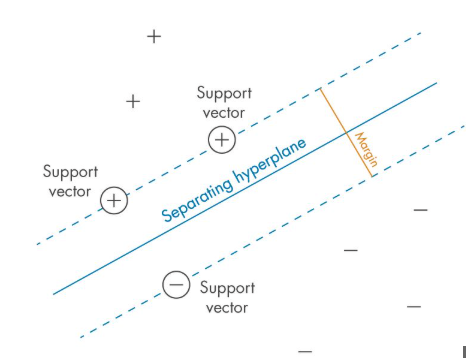
\includegraphics[width=0.3\textwidth]{Figures/SVM1.png}
                \caption{Hiperplano separador con margen máximo}
            \end{figure}
        \end{center}
\end{frame}

\begin{frame}{El Problema de Clasificación Lineal}
    \begin{block}{Escenario básico}
        Sea un conjunto de datos $\{(\mathbf{x}_i, y_i)\}_{i=1}^{N}$ donde:
        \begin{itemize}
            \item $\mathbf{x}_i \in \mathbb{R}^d$ — vector de características
            \item $y_i \in \{-1, +1\}$ — etiqueta de clase
        \end{itemize}
    \end{block}

    \vspace{0.4em}

    \begin{columns}
        \column{0.5\textwidth}
        \textbf{Clasificador lineal genérico:}
        \begin{equation}
            f(\mathbf{x}) = \text{sign}(\mathbf{w}^\top \mathbf{x} + b)
        \end{equation}
        \begin{itemize}
            \item $\mathbf{w}$ — vector normal al hiperplano
            \item $b$ — término de sesgo (\textit{bias})
        \end{itemize}

        \column{0.5\textwidth}
        \begin{alertblock}{Problema de ambigüedad}
            Pueden existir \textbf{infinitos hiperplanos} separadores. ¿Cuál elegir?
        \end{alertblock}
        \vspace{0.3em}
        $\Rightarrow$ SVM responde: el que \textbf{maximiza el margen}.
    \end{columns}
\end{frame}

%------------------------------------------------
\section{Hiperplano de Margen Máximo}
%------------------------------------------------

\begin{frame}{Concepto de Margen}
    \begin{columns}
        \column{0.55\textwidth}
        \begin{block}{Definición de margen}
            El \textbf{margen} es la distancia entre el hiperplano separador y los puntos más cercanos de cada clase.
        \end{block}
        La distancia de un punto $\mathbf{x}_i$ al hiperplano es:
        \begin{equation}
            d_i = \frac{y_i \, (\mathbf{w}^\top \mathbf{x}_i + b)}{\|\mathbf{w}\|}
        \end{equation}
        El margen total es:
        \begin{equation}
            \rho = \frac{2}{\|\mathbf{w}\|}
        \end{equation}

        \column{0.42\textwidth}
        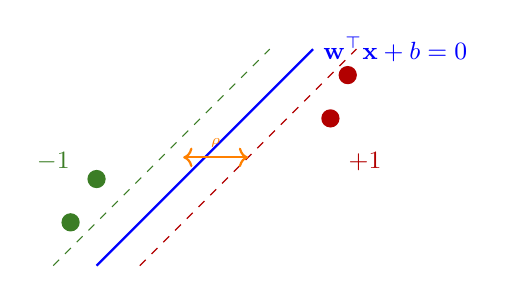
\begin{tikzpicture}[scale=1.1]
            % Hyperplane
            \draw[thick, blue] (0,0) -- (2.5,2.5) node[right]{\small $\mathbf{w}^\top\mathbf{x}+b=0$};
            % Margin lines
            \draw[dashed, OliveGreen] (-0.5,0) -- (2.0,2.5);
            \draw[dashed, red!70!black] (0.5,0) -- (3.0,2.5);
            % Support vectors class +1
            \fill[red!70!black] (2.9,2.2) circle (3pt);
            \fill[red!70!black] (2.7,1.7) circle (3pt);
            % Support vectors class -1
            \fill[OliveGreen] (-0.3,0.5) circle (3pt);
            \fill[OliveGreen] (0.0,1.0) circle (3pt);
            % Margin arrow
            \draw[<->,thick,orange] (1.0,1.25) -- (1.75,1.25) node[midway,above]{\tiny $\rho$};
            % Labels
            \node[red!70!black] at (3.1,1.2) {\small $+1$};
            \node[OliveGreen] at (-0.5,1.2) {\small $-1$};
        \end{tikzpicture}
    \end{columns}
\end{frame}

\begin{frame}{Vectores de Soporte}
    \begin{block}{Definición de \textit{Support Vectors}}
        Los \textbf{vectores de soporte} son los puntos de entrenamiento que se encuentran exactamente sobre los hiperplanos de margen:
        \begin{equation}
            \mathbf{w}^\top \mathbf{x}_i + b = \pm 1
        \end{equation}
        Son los únicos puntos que \textbf{definen el hiperplano óptimo}.
    \end{block}

    \vspace{0.3em}

    \begin{columns}
        \column{0.5\textwidth}
        \begin{exampleblock}{Propiedad clave}
            Si se eliminan todos los puntos de entrenamiento \textbf{excepto} los vectores de soporte, el hiperplano óptimo no cambia.
        \end{exampleblock}

        \column{0.5\textwidth}
        \begin{alertblock}{Implicación práctica}
            SVM es \textbf{eficiente en memoria}: solo almacena los vectores de soporte, no todo el conjunto de entrenamiento.
        \end{alertblock}
    \end{columns}
\end{frame}

\begin{frame}{Formulación del Problema de Optimización}
    \begin{block}{Problema primal — caso separable}
        Maximizar el margen $\rho = 2/\|\mathbf{w}\|$ es equivalente a:
    \end{block}

    \begin{equation}
        \min_{\mathbf{w},\,b} \quad \frac{1}{2}\|\mathbf{w}\|^2
    \end{equation}

    \textbf{sujeto a:}
    \begin{equation}
        y_i \, (\mathbf{w}^\top \mathbf{x}_i + b) \geq 1, \quad \forall \, i = 1, \ldots, N
    \end{equation}

    \begin{itemize}
        \item $\|\mathbf{w}\|^2 = \mathbf{w}^\top \mathbf{w}$ — norma euclidiana al cuadrado
        \item Las restricciones garantizan que todos los puntos estén correctamente clasificados con margen $\geq 1$
        \item Es un problema de \textbf{programación cuadrática convexa} (QP) — solución única y global
    \end{itemize}
\end{frame}

%------------------------------------------------
\section{Formulación Dual y Multiplicadores de Lagrange}
%------------------------------------------------

\begin{frame}{El Lagrangiano del Problema Primal}
    Para resolver el problema con restricciones, se introduce el \textbf{Lagrangiano}:

    \begin{equation}
        \mathcal{L}(\mathbf{w}, b, \boldsymbol{\alpha}) = \frac{1}{2}\|\mathbf{w}\|^2 - \sum_{i=1}^{N} \alpha_i \left[ y_i(\mathbf{w}^\top \mathbf{x}_i + b) - 1 \right]
    \end{equation}

    \begin{itemize}
        \item $\alpha_i \geq 0$ — multiplicadores de Lagrange (uno por muestra)
        \item Se aplican las condiciones \textbf{KKT} (\textit{Karush-Kuhn-Tucker})
    \end{itemize}
\end{frame}
\begin{frame}{El Lagrangiano del Problema Primal}
    \begin{block}{Condiciones KKT de optimalidad}
        \begin{equation}
            \frac{\partial \mathcal{L}}{\partial \mathbf{w}} = 0 \Rightarrow \mathbf{w} = \sum_{i=1}^{N} \alpha_i y_i \mathbf{x}_i
        \end{equation}
        \begin{equation}
            \frac{\partial \mathcal{L}}{\partial b} = 0 \Rightarrow \sum_{i=1}^{N} \alpha_i y_i = 0
        \end{equation}
    \end{block}
\end{frame}

\begin{frame}{Problema Dual}
    Sustituyendo las condiciones KKT en el Lagrangiano se obtiene el \textbf{problema dual}:

    \begin{equation}
        \max_{\boldsymbol{\alpha}} \quad W(\boldsymbol{\alpha}) = \sum_{i=1}^{N} \alpha_i - \frac{1}{2} \sum_{i=1}^{N} \sum_{j=1}^{N} \alpha_i \alpha_j y_i y_j \, \mathbf{x}_i^\top \mathbf{x}_j
    \end{equation}

    \textbf{sujeto a:}
    \begin{equation}
        \alpha_i \geq 0, \quad \sum_{i=1}^{N} \alpha_i y_i = 0
    \end{equation}
\end{frame}
\begin{frame}{Problema Dual}

    \begin{columns}
        \column{0.5\textwidth}
        \begin{block}{Holgura complementaria (KKT)}
            \begin{equation}
                \alpha_i \left[ y_i(\mathbf{w}^\top \mathbf{x}_i + b) - 1 \right] = 0
            \end{equation}
            Si $\alpha_i > 0$ $\Rightarrow$ punto es vector de soporte.
        \end{block}

        \column{0.5\textwidth}
        \begin{exampleblock}{Ventaja del dual}
            El problema dual depende solo de \textbf{productos internos} $\mathbf{x}_i^\top \mathbf{x}_j$, lo que facilita la extensión mediante \textbf{funciones Kernel}.
        \end{exampleblock}
    \end{columns}
\end{frame}

\begin{frame}{Clasificación con el Modelo Entrenado}
    Una vez resuelto el dual, se obtiene:

    \begin{equation}
        \mathbf{w}^* = \sum_{i \in SV} \alpha_i^* \, y_i \, \mathbf{x}_i
    \end{equation}

    \begin{equation}
        b^* = y_k - \mathbf{w}^{*\top} \mathbf{x}_k \quad \text{para cualquier vector de soporte } \mathbf{x}_k
    \end{equation}

    La función de decisión para un nuevo punto $\mathbf{x}$ es:

    \begin{equation}
        f(\mathbf{x}) = \text{sign}\left( \sum_{i \in SV} \alpha_i^* \, y_i \, \mathbf{x}_i^\top \mathbf{x} + b^* \right)
    \end{equation}
\end{frame}
\begin{frame}{Clasificación con el Modelo Entrenado}

    \begin{alertblock}{Observación importante}
        La clasificación se realiza únicamente sobre los \textbf{vectores de soporte} (donde $\alpha_i^* > 0$). Puntos con $\alpha_i^* = 0$ no participan.
    \end{alertblock}
\end{frame}

%------------------------------------------------
\section{SVM de Margen Suave (Soft Margin)}
%------------------------------------------------

\begin{frame}{Datos No Separables Linealmente}
    \begin{columns}
        \column{0.55\textwidth}
        \begin{block}{Problema con el caso rígido}
            En la práctica, los datos raramente son \textbf{linealmente separables}. El problema de margen duro no tiene solución en presencia de ruido u \textit{outliers}.
        \end{block}
        \vspace{0.3em}
        \textbf{Solución:} introducir variables de holgura $\xi_i \geq 0$ que permitan violaciones del margen:
        \begin{equation}
            y_i (\mathbf{w}^\top \mathbf{x}_i + b) \geq 1 - \xi_i
        \end{equation}

        \column{0.42\textwidth}
        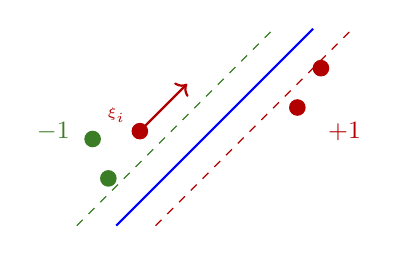
\begin{tikzpicture}[scale=1.0]
            \draw[thick, blue] (0.2,0) -- (2.7,2.5);
            \draw[dashed, OliveGreen] (-0.3,0) -- (2.2,2.5);
            \draw[dashed, red!70!black] (0.7,0) -- (3.2,2.5);
            \fill[red!70!black] (2.8,2.0) circle (3pt);
            \fill[red!70!black] (2.5,1.5) circle (3pt);
            % Outlier cross margin
            \fill[red!70!black] (0.5,1.2) circle (3pt);
            \node[red!70!black, font=\tiny] at (0.2,1.4) {$\xi_i$};
            \draw[->, red!70!black, thick] (0.5,1.2) -- (1.1,1.8);
            \fill[OliveGreen] (0.1,0.6) circle (3pt);
            \fill[OliveGreen] (-0.1,1.1) circle (3pt);
            \node[red!70!black] at (3.1,1.2) {\small $+1$};
            \node[OliveGreen] at (-0.6,1.2) {\small $-1$};
        \end{tikzpicture}
    \end{columns}
\end{frame}

\begin{frame}{Formulación del Margen Suave}
    \begin{block}{Problema primal — \textit{Soft Margin} SVM}
        \begin{equation}
            \min_{\mathbf{w},\,b,\,\boldsymbol{\xi}} \quad \frac{1}{2}\|\mathbf{w}\|^2 + C \sum_{i=1}^{N} \xi_i
        \end{equation}
        \textbf{sujeto a:}
        \begin{equation}
            y_i(\mathbf{w}^\top \mathbf{x}_i + b) \geq 1 - \xi_i, \quad \xi_i \geq 0, \quad \forall \, i
        \end{equation}
    \end{block}
\end{frame}
\begin{frame}{Formulación del Margen Suave}

    \begin{columns}
        \column{0.5\textwidth}
        \begin{itemize}
            \item $\xi_i$ — variable de holgura del punto $i$
            \item $C > 0$ — parámetro de regularización
            \item $\xi_i = 0$: punto clasificado correctamente
            \item $0 < \xi_i \leq 1$: dentro del margen
            \item $\xi_i > 1$: clasificado incorrectamente
        \end{itemize}

        \column{0.5\textwidth}
        \begin{alertblock}{Rol del parámetro $C$}
            \begin{itemize}
                \item $C$ grande $\Rightarrow$ penaliza errores (\textit{hard margin})
                \item $C$ pequeño $\Rightarrow$ tolera violaciones (\textit{soft margin})
                \item $C$ se ajusta por \textbf{validación cruzada}
            \end{itemize}
        \end{alertblock}
    \end{columns}
\end{frame}

\begin{frame}{Problema Dual del Margen Suave}
    El problema dual del \textit{Soft Margin} es:

    \begin{equation}
        \max_{\boldsymbol{\alpha}} \quad \sum_{i=1}^{N} \alpha_i - \frac{1}{2} \sum_{i=1}^{N} \sum_{j=1}^{N} \alpha_i \alpha_j y_i y_j \, \mathbf{x}_i^\top \mathbf{x}_j
    \end{equation}

    \textbf{sujeto a:}
    \begin{equation}
        0 \leq \alpha_i \leq C, \quad \sum_{i=1}^{N} \alpha_i y_i = 0
    \end{equation}
\end{frame}
\begin{frame}{Problema Dual del Margen Suave}

    \begin{block}{Comparación con el margen duro}
        \begin{center}
        \begin{tabular}{lccc}
            \toprule
            Formulación & Restricción en $\alpha_i$ & Tolerancia a ruido \\
            \midrule
            Margen Duro & $\alpha_i \geq 0$ & No \\
            Margen Suave & $0 \leq \alpha_i \leq C$ & Sí \\
            \bottomrule
        \end{tabular}
        \end{center}
        La única diferencia es la cota superior $C$ en los multiplicadores.
    \end{block}
\end{frame}

%------------------------------------------------
\section{El Truco del Kernel}
%------------------------------------------------

\begin{frame}{Limitaciones del Clasificador Lineal}
    \begin{columns}
        \column{0.5\textwidth}
        \begin{block}{Problema con datos no lineales}
            Muchos problemas reales \textbf{no son linealmente separables} en el espacio original $\mathbb{R}^d$.
        \end{block}
        \vspace{0.3em}
        \textbf{Idea:} mapear los datos a un espacio de mayor dimensión $\mathcal{H}$ donde sí sean separables:
        \begin{equation}
            \phi: \mathbb{R}^d \rightarrow \mathcal{H}
        \end{equation}
        Se aplica SVM lineal en $\mathcal{H}$.

        \column{0.5\textwidth}
        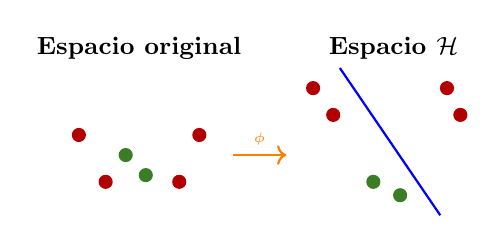
\begin{tikzpicture}[scale=0.85]
            % Original space (not separable)
            \node[font=\small\bfseries] at (1.2,2.8) {Espacio original};
            \fill[red!70!black] (0.3,1.5) circle (3pt);
            \fill[red!70!black] (0.7,0.8) circle (3pt);
            \fill[red!70!black] (2.1,1.5) circle (3pt);
            \fill[red!70!black] (1.8,0.8) circle (3pt);
            \fill[OliveGreen] (1.0,1.2) circle (3pt);
            \fill[OliveGreen] (1.3,0.9) circle (3pt);
            % Arrow
            \draw[->, thick, orange] (2.6,1.2) -- (3.4,1.2) node[midway,above]{\tiny $\phi$};
            % Mapped space (separable)
            \node[font=\small\bfseries] at (5.0,2.8) {Espacio $\mathcal{H}$};
            \fill[red!70!black] (3.8,2.2) circle (3pt);
            \fill[red!70!black] (4.1,1.8) circle (3pt);
            \fill[red!70!black] (5.8,2.2) circle (3pt);
            \fill[red!70!black] (6.0,1.8) circle (3pt);
            \fill[OliveGreen] (4.7,0.8) circle (3pt);
            \fill[OliveGreen] (5.1,0.6) circle (3pt);
            \draw[thick, blue] (4.2,2.5) -- (5.7,0.3);
        \end{tikzpicture}
    \end{columns}
\end{frame}

\begin{frame}{El Truco del Kernel}
    \begin{block}{Observación fundamental}
        El problema dual SVM solo depende de \textbf{productos internos}:
        \begin{equation}
            \mathbf{x}_i^\top \mathbf{x}_j \quad \Longrightarrow \quad \phi(\mathbf{x}_i)^\top \phi(\mathbf{x}_j)
        \end{equation}
    \end{block}

    \begin{exampleblock}{Función Kernel}
        Se define la función Kernel como:
        \begin{equation}
            K(\mathbf{x}_i, \mathbf{x}_j) = \phi(\mathbf{x}_i)^\top \phi(\mathbf{x}_j)
        \end{equation}
        El \textbf{truco del kernel} permite calcular el producto interno en $\mathcal{H}$ \textbf{sin calcular explícitamente} $\phi(\mathbf{x})$.
    \end{exampleblock}

    \begin{alertblock}{Consecuencia práctica}
        Solo se necesita definir $K(\cdot,\cdot)$, no la función $\phi$ explícitamente. El costo computacional no depende de la dimensión de $\mathcal{H}$ (que puede ser infinita).
    \end{alertblock}
\end{frame}

\begin{frame}{Kernels Más Utilizados}
    La función de decisión con kernel queda:
    \begin{equation}
        f(\mathbf{x}) = \text{sign}\left( \sum_{i \in SV} \alpha_i^* \, y_i \, K(\mathbf{x}_i, \mathbf{x}) + b^* \right)
    \end{equation}

    \vspace{0.4em}
    \begin{center}
    \begin{tabular}{lll}
        \toprule
        \textbf{Kernel} & \textbf{Fórmula} $K(\mathbf{x}_i, \mathbf{x}_j)$ & \textbf{Parámetros} \\
        \midrule
        Lineal        & $\mathbf{x}_i^\top \mathbf{x}_j$ & — \\[4pt]
        Polinomial    & $(\mathbf{x}_i^\top \mathbf{x}_j + c)^d$ & $c \geq 0$, $d \in \mathbb{Z}^+$ \\[4pt]
        RBF (Gaussiano) & $\exp\!\left(-\gamma\|\mathbf{x}_i - \mathbf{x}_j\|^2\right)$ & $\gamma > 0$ \\[4pt]
        Sigmoide      & $\tanh(\kappa\,\mathbf{x}_i^\top \mathbf{x}_j + \theta)$ & $\kappa,\theta$ \\
        \bottomrule
    \end{tabular}
    \end{center}
\end{frame}
\begin{frame}{Kernels Más Utilizados}

    \begin{exampleblock}{Condición de Mercer}
        Una función $K$ es un kernel válido si y solo si la matriz de Gram $K_{ij} = K(\mathbf{x}_i,\mathbf{x}_j)$ es \textbf{semidefinida positiva}.
    \end{exampleblock}
\end{frame}

\begin{frame}{Kernel RBF: Intuición Geométrica}
    El kernel \textbf{RBF} (\textit{Radial Basis Function}) o Gaussiano es el más empleado en la práctica:

    \begin{equation}
        K(\mathbf{x}_i, \mathbf{x}_j) = \exp\!\left(-\gamma\|\mathbf{x}_i - \mathbf{x}_j\|^2\right), \quad \gamma > 0
    \end{equation}

    \begin{columns}
        \column{0.5\textwidth}
        \begin{block}{Interpretación}
            Mide la \textbf{similitud} entre dos puntos: decrece exponencialmente con la distancia al cuadrado entre ellos.
        \end{block}
        \begin{itemize}
            \item $\gamma$ pequeño $\Rightarrow$ vecindad amplia (\textit{underfitting})
            \item $\gamma$ grande $\Rightarrow$ vecindad estrecha (\textit{overfitting})
        \end{itemize}

        \column{0.5\textwidth}
        \begin{alertblock}{Selección de hiperparámetros}
            Para SVM con RBF se ajustan \textbf{dos parámetros}:
            \begin{itemize}
                \item $C$ — regularización del margen
                \item $\gamma$ — radio del kernel
            \end{itemize}
            Se recomienda búsqueda en grilla logarítmica con \textbf{validación cruzada} $k$-fold.
        \end{alertblock}
    \end{columns}
\end{frame}

%------------------------------------------------
\section{SVM Multi-clase y SVR}
%------------------------------------------------

\begin{frame}{Extensión a Multi-clase}
    \begin{block}{SVM binario $\rightarrow$ multi-clase}
        SVM es inherentemente \textbf{binario}. Se extiende a $K$ clases mediante estrategias combinatorias.
    \end{block}

    \vspace{0.3em}
    \begin{columns}
        \column{0.5\textwidth}
        \textbf{Uno contra el resto (OvR):}
        \begin{itemize}
            \item $K$ clasificadores SVM
            \item El clasificador $k$ separa la clase $k$ de todas las demás
            \item Se asigna la clase con mayor valor de $f_k(\mathbf{x})$
        \end{itemize}
        \vspace{0.3em}
        \textbf{Complejidad:} $K$ problemas QP

        \column{0.5\textwidth}
        \textbf{Uno contra uno (OvO):}
        \begin{itemize}
            \item $\binom{K}{2}$ clasificadores SVM
            \item Cada clasificador separa un par de clases
            \item Se asigna la clase por \textbf{votación mayoritaria}
        \end{itemize}
        \vspace{0.3em}
        \textbf{Complejidad:} $K(K-1)/2$ problemas QP
    \end{columns}
\end{frame}
\begin{frame}{Extensión a Multi-clase}

    \vspace{0.3em}
    \begin{exampleblock}{Recomendación práctica}
        OvO es más común en implementaciones (e.g., MATLAB, scikit-learn) por su mejor estabilidad numérica con clases desbalanceadas.
    \end{exampleblock}
\end{frame}

\begin{frame}{Support Vector Regression (SVR)}
    SVM puede adaptarse para \textbf{regresión} con la formulación $\epsilon$-SVR:

    \begin{equation}
        \min_{\mathbf{w},b,\boldsymbol{\xi}} \quad \frac{1}{2}\|\mathbf{w}\|^2 + C \sum_{i=1}^{N} (\xi_i + \xi_i^*)
    \end{equation}

    \textbf{sujeto a:}
    \begin{equation}
        |y_i - (\mathbf{w}^\top\mathbf{x}_i + b)| \leq \epsilon + \xi_i^{(*)}
    \end{equation}

    \begin{columns}
        \column{0.5\textwidth}
        \begin{block}{Tubo $\epsilon$-insensible}
            Las predicciones dentro del tubo de ancho $2\epsilon$ \textbf{no generan error}. Solo los puntos fuera del tubo contribuyen a la función objetivo.
        \end{block}

        \column{0.5\textwidth}
        \begin{itemize}
            \item $\epsilon$ — anchura del tubo de tolerancia
            \item $C$ — regularización (igual que en clasificación)
            \item $\xi_i, \xi_i^*$ — holguras superior e inferior
        \end{itemize}
    \end{columns}
\end{frame}

%------------------------------------------------
\section{Implementación en MATLAB}
%------------------------------------------------

\begin{frame}[fragile]{SVM Binario en MATLAB — Entrenamiento}
\begin{lstlisting}[language=Matlab, style=MATLABStyle]
% Cargar o generar datos
load fisheriris;
X = meas(51:end, 1:2);        % 2 caracteristicas, 2 clases
Y = categorical(species(51:end));

% Dividir en entrenamiento/prueba (70/30)
cv = cvpartition(Y, 'HoldOut', 0.3);
X_train = X(cv.training, :);
Y_train = Y(cv.training);
X_test  = X(cv.test, :);
Y_test  = Y(cv.test);

% Entrenar SVM con kernel RBF
svmModel = fitcsvm(X_train, Y_train, ...
    'KernelFunction', 'rbf', ...
    'BoxConstraint',   1, ...       % parametro C
    'KernelScale',    'auto', ...   % gamma automatico
    'Standardize',    true);

disp('Entrenamiento completado.');
disp(['Numero de vectores de soporte: ', ...
      num2str(sum(svmModel.IsSupportVector))]);
\end{lstlisting}
\end{frame}

\begin{frame}[fragile]{SVM Binario en MATLAB — Evaluación}
\begin{lstlisting}[language=Matlab, style=MATLABStyle]
% Prediccion en conjunto de prueba
Y_pred = predict(svmModel, X_test);

% Matriz de confusion
confMat = confusionmat(Y_test, Y_pred);
disp('Matriz de confusion:'); disp(confMat);

% Metricas de desempeno
accuracy = sum(Y_pred == Y_test) / numel(Y_test) * 100;
fprintf('Exactitud: %.2f%%\n', accuracy);

% Visualizar frontera de decision
figure;
h = 0.02;
[x1g, x2g] = meshgrid(...
    min(X(:,1))-1:h:max(X(:,1))+1, ...
    min(X(:,2))-1:h:max(X(:,2))+1);
Xgrid = [x1g(:), x2g(:)];
[~, scores] = predict(svmModel, Xgrid);
contourf(x1g, x2g, reshape(scores(:,2),size(x1g)), ...
    'LineColor','none');
colormap cool; colorbar;
hold on;
gscatter(X(:,1), X(:,2), Y, 'rb', '.o', 8);
title('Frontera de decision SVM (RBF)');
xlabel('Caracteristica 1'); ylabel('Caracteristica 2');
\end{lstlisting}
\end{frame}

\begin{frame}[fragile]{Selección de Hiperparámetros con Búsqueda en Grilla}
\begin{lstlisting}[language=Matlab, style=MATLABStyle]
% Grilla logaritmica de C y gamma
C_grid     = logspace(-2, 3, 12);   % 0.01 a 1000
gamma_grid = logspace(-4, 1, 12);   % 0.0001 a 10

best_acc = 0;
best_C = 1; best_g = 1;

for C = C_grid
    for g = gamma_grid
        mdl = fitcsvm(X_train, Y_train, ...
            'KernelFunction', 'rbf', ...
            'BoxConstraint',   C, ...
            'KernelScale',     1/sqrt(2*g), ...
            'Standardize',     true, ...
            'CrossVal',        'on', ...
            'KFold',           5);
        acc = 1 - kfoldLoss(mdl);
        if acc > best_acc
            best_acc = acc;
            best_C = C; best_g = g;
        end
    end
end
fprintf('Optimos: C=%.4f, gamma=%.4f, Acc=%.2f%%\n', ...
        best_C, best_g, best_acc*100);
\end{lstlisting}
\end{frame}

\begin{frame}[fragile]{SVR en MATLAB}
\begin{lstlisting}[language=Matlab, style=MATLABStyle]
% Datos de regresion: prediccion de precio
% X = caracteristicas, y = variable objetivo continua
load carsmall
X_reg = [Horsepower, Weight];
y_reg = MPG;

% Eliminar filas con NaN
idx = ~any(isnan([X_reg, y_reg]), 2);
X_reg = X_reg(idx,:); y_reg = y_reg(idx);

% Entrenar epsilon-SVR
svrModel = fitrsvm(X_reg, y_reg, ...
    'KernelFunction', 'rbf', ...
    'BoxConstraint',   10, ...       % C
    'Epsilon',         0.1, ...      % epsilon del tubo
    'KernelScale',    'auto', ...
    'Standardize',    true);

% Evaluar con RMSE
y_pred = predict(svrModel, X_reg);
rmse = sqrt(mean((y_pred - y_reg).^2));
fprintf('RMSE en entrenamiento: %.4f\n', rmse);
fprintf('Vectores de soporte: %d\n', ...
        sum(svrModel.IsSupportVector));
\end{lstlisting}
\end{frame}

%------------------------------------------------
\section{Ventajas, Limitaciones y Comparativa}
%------------------------------------------------

\begin{frame}{Ventajas y Limitaciones de SVM}
    \begin{columns}
        \column{0.5\textwidth}
        \textbf{\color{OliveGreen}Ventajas:}
        \begin{itemize}
            \item Efectivo en \textbf{alta dimensionalidad}
            \item Eficiente en memoria (solo vectores de soporte)
            \item Garantías teóricas sólidas (\textit{VC dimension})
            \item Flexible mediante elección de kernel
            \item Robusto ante \textit{overfitting} (margen máximo)
            \item Único mínimo global (problema convexo)
        \end{itemize}

        \column{0.5\textwidth}
        \textbf{\color{red!70!black}Limitaciones:}
        \begin{itemize}
            \item Costoso en entrenamiento: $\mathcal{O}(N^2)$ a $\mathcal{O}(N^3)$
            \item No escala bien a millones de muestras
            \item Selección de kernel y $C$, $\gamma$ es crítica
            \item No produce probabilidades directamente
            \item Sensible a la escala de las características
            \item Difícil interpretación (caja negra con kernel)
        \end{itemize}
    \end{columns}
\end{frame}
\begin{frame}{Ventajas y Limitaciones de SVM}

    \vspace{0.3em}
    \begin{alertblock}{Regla de escala}
        \textbf{Siempre normalizar} las características antes de entrenar un SVM. La distancia euclidiana (y el kernel RBF) es sensible a la magnitud de las variables.
    \end{alertblock}
\end{frame}

\begin{frame}{SVM vs. Otras Técnicas de Clasificación}
    \begin{center}
    \begin{tabular}{lccccc}
        \toprule
        \textbf{Método} & \textbf{Lineal} & \textbf{Kernel} & \textbf{Escala} & \textbf{Probabilidades} & \textbf{Interpretable} \\
        \midrule
        SVM (lineal)    & Sí & No  & Media  & No  & Medio \\
        SVM (RBF)       & No & Sí  & Media  & No  & Bajo \\
        Regresión Log.  & Sí & No  & Alta   & Sí  & Alto \\
        Árbol de dec.   & No & No  & Alta   & Sí  & Alto \\
        Random Forest   & No & No  & Alta   & Sí  & Bajo \\
        Red Neuronal    & No & No  & Media  & Sí  & Muy bajo \\
        \bottomrule
    \end{tabular}
    \end{center}
\end{frame}
\begin{frame}{SVM vs. Otras Técnicas de Clasificación}

    \begin{exampleblock}{Cuando SVM es preferible}
        \begin{itemize}
            \item Datos con alta relación dimensiones/muestras ($d \gg N$)
            \item Problemas con estructura clara de separación pero no lineal
            \item Cuando se requieren garantías teóricas de generalización
        \end{itemize}
    \end{exampleblock}
\end{frame}

%------------------------------------------------
\section{Resumen y Referencias}
%------------------------------------------------

\begin{frame}{Resumen del Módulo}
        \textbf{Conceptos clave cubiertos:}
        \begin{enumerate}
            \footnotesize
            \item Hiperplano de margen máximo
            \item Vectores de soporte
            \item Formulación primal y dual (Lagrangiano + KKT)
            \item \textit{Soft Margin} y parámetro $C$
            \item Truco del Kernel y condición de Mercer
            \item Kernels: lineal, polinomial, RBF, sigmoide
            \item SVM multi-clase: OvR y OvO
            \item \textit{Support Vector Regression} (SVR)
            \item Implementación en MATLAB
        \end{enumerate}
    \end{frame}
    \begin{frame}{Resumen del Módulo}

        \begin{alertblock}{Fórmula central — Función de decisión}
            \begin{equation*}
                f(\mathbf{x}) = \text{sign}\!\left(\sum_{i \in SV} \alpha_i^* y_i K(\mathbf{x}_i, \mathbf{x}) + b^*\right)
            \end{equation*}
        \end{alertblock}
        \vspace{0.3em}
        \begin{block}{Flujo de trabajo SVM}
            \begin{enumerate}
                \item Normalizar datos
                \item Seleccionar kernel
                \item Ajustar $C$ y $\gamma$ (CV $k$-fold)
                \item Entrenar y evaluar
                \item Interpretar vectores de soporte
            \end{enumerate}
        \end{block}
\end{frame}

\begin{frame}{Referencias}
    \begin{exampleblock}{Textos fundamentales}
        \begin{itemize}
            \item \textbf{Cortes \& Vapnik (1995).} Support-Vector Networks. \textit{Machine Learning}, 20(3), 273--297.
            \item \textbf{Vapnik, V. (1998).} \textit{Statistical Learning Theory}. Wiley-Interscience.
            \item \textbf{Schölkopf \& Smola (2002).} \textit{Learning with Kernels}. MIT Press.
            \item \textbf{Bishop, C.M. (2006).} \textit{Pattern Recognition and Machine Learning}. Springer. Cap. 7.
        \end{itemize}
    \end{exampleblock}
\end{frame}
\begin{frame}{Referencias}

    \vspace{0.3em}
    \begin{exampleblock}{Documentación MATLAB}
        \begin{itemize}
            \item \url{https://www.mathworks.com/help/stats/fitcsvm.html}
            \item \url{https://www.mathworks.com/help/stats/fitrsvm.html}
        \end{itemize}
    \end{exampleblock}
\end{frame}

\end{document}